\chapter{Metodologia}
% Label para referenciar
\label{metodologia}
O estudo apresenta a modelagem e implementação de uma arquitetura que possibilite a extração, processamento e disponibilização dos dados referente à Câmara dos Deputados. Este projeto foi desenvolvido utilizando o Databricks, que pode ser definida como uma plataforma unificada para análise de dados na \textit{Cloud} para um volume massivo de dados, promovendo a colaboração entre Cientistas e Engenheiros de Dados\footnote{Disponível em <https://databricks.com/product/unified-data-analytics-platform> Acesso em: 19 mai, 2020}.
A arquitetura pode ser definida em 3 camadas (serão detalhadas nas seções a seguir):
\begin{enumerate} 
 \item [1)] Armazenamento;
 \item [2)] \textit{Extract, Transform and Load (ETL)};
 \item [3)] Análise exploratória de dados.
\end{enumerate} 

Pode-se ter uma visão do fluxo de processamento na figura 4.

% Figura
\begin{figure}[H]
	\centering	
	\caption[\hspace{0.1cm}Arquitetura proposta]{Arquitetura proposta}
	  \vspace{-0.4cm}
	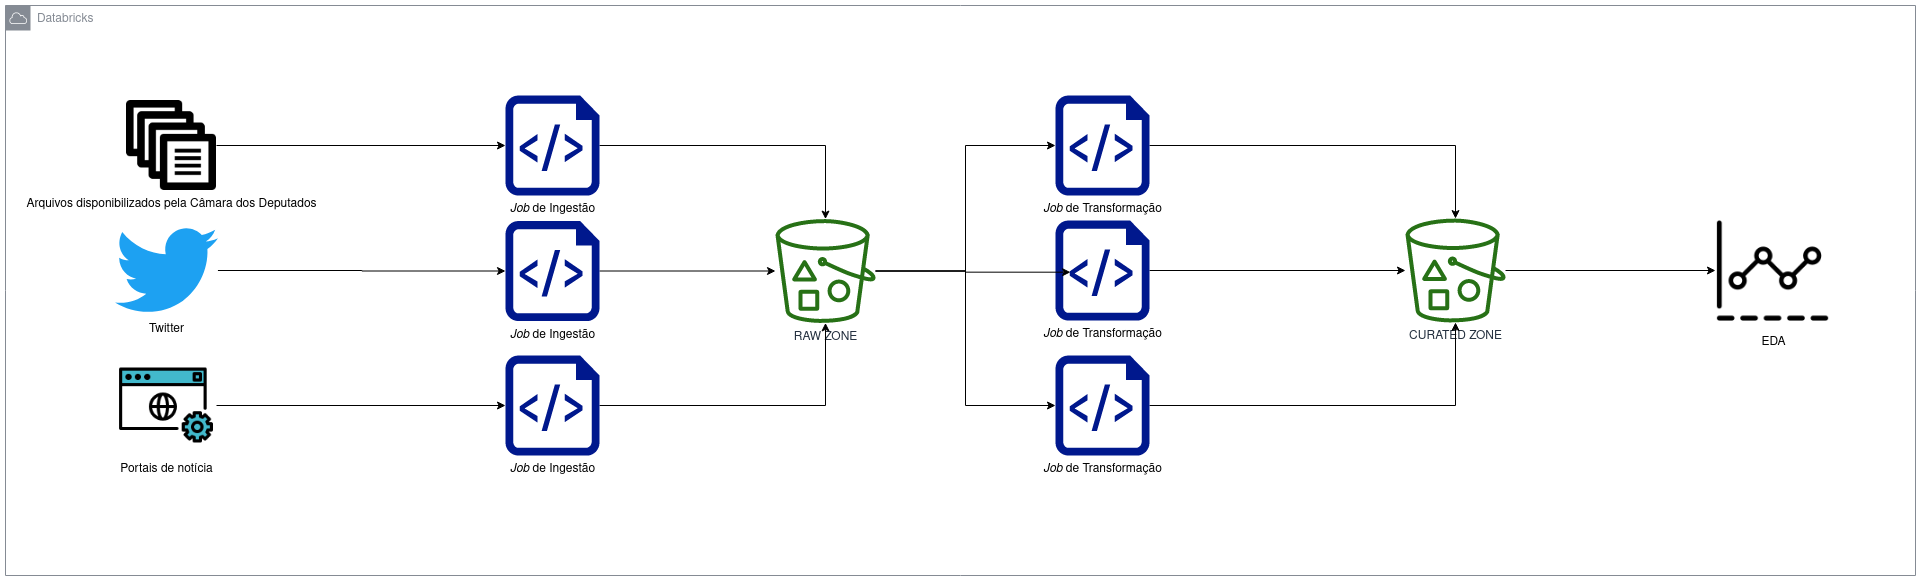
\includegraphics[width=.8\textwidth]{figuras/tcc_arch.png}
	% Caption centralizada
% 	\captionsetup{justification=centering}
	% Caption e fonte
	 \vspace{-0.3cm}
	\\\textbf{\footnotesize Fonte: Elaborada pelo autor}
	\label{fig:tela1}
\end{figure}

\section{Armazenamento} O Databricks está sendo utilizado como plataforma unificada do projeto, o que inclui o seu armazenamento. Uma das funcionalidades disponíveis é o \textit{file system} distribuído para armazenamento de dados em sua plataforma. É denominado como \textit{Databricks File System (DBFS)} e é compartilhado por todos os nós do \textit{cluster}\footnote{Disponível em <hhttps://docs.databricks.com/data/databricks-file-system.html> Acesso em: 19 mai, 2020}. Uma arquitetura de \textit{Data Lake} está sendo utilizada, logo temos a segmentação dos dados em zonas. Os dados originais são armazenados na \textit{Raw zone} em seu formato original. Após os processos de ETL, os dados já tratados são armazenados na \textit{Curated zone} em formato parquet, uma vez que este formato de armazenamento colunar é otimizado para o uso com o Spark e diminui drasticamente o espaço em disco necessário\footnote{Disponível em <https://parquet.apache.org/> Acesso em: 19 mai, 2020}.

\section{\textit{Extract, Transform and Load (ETL)}} Todo o processamento deste projeto foi realizado utilizando o Apache Spark. Este processamento foi segmentado em duas etapas, sendo elas:

\subsection{Ingestão de dados} Essa camada tem como objetivo o detalhamento dos processos que extraem os dados de sua fonte originária e os inserem, sem maiores tratamentos, no ambiente analítico. Foram elencadas 3 fontes de dados para o projeto, sendo elas:

\subsubsection{Dados Abertos da Câmara dos Deputados} A fonte oficial de dados da Câmara dos Deputados. Tratam-se de arquivos históricos disponibilizados pelo Câmara que contém todas as informações pessoais e políticas dos parlamentares, além dos históricos de reembolsos, discursos políticos, votações, emendas de sua autoria ou co-participação, entre diversas outras informações referentes à sua atividade parlamentar\footnote{Disponível em <https://dadosabertos.camara.leg.br/> Acesso em: 19 mai, 2020}. Os arquivos de 2009 a 2019 foram extraídos manualmente e inseridos na \textit{Raw zone} do nosso \textit{Data Lake}. Para este projeto, os dados dos seguintes temas foram extraídos:

\begin{itemize}
\item \textbf{Dados dos Deputados}: Deputados que já estiveram em exercício na Câmara dos Deputados;
\item \textbf{Despesas dos parlamentares}: Despesas referentes ao exercício da Atividade Parlamentar de cada deputado;
\item \textbf{Proposições}: Proposições apresentadas à Câmara dos Deputados com suas respectivas informações;
\item \textbf{Autores das Proposições}: Autores das proposições submetidas à Câmara;
\item \textbf{Classificação temática das proposições}: Informações mais detalhadas referentes aos temas das proposições submetidas.
\end{itemize}

\subsubsection{API do Twitter} O Twitter é uma rede social criada em 15 de julho de 2006 e, em fevereiro de 2019, possuia 321 milhões de usuários ativos\footnote{Disponível em <https://pt.wikipedia.org/wiki/Twitter> Acesso em: 19 mai, 2020}.Para extrair os \textit{tweets} desta plataforma, foi criado um \textit{job} utilizando Python e Spark e um módulo de comunicação com Twitter, o tweepy, que é caracterizado pelos autores como uma biblioteca de fácil uso para acesso à API do Twitter\footnote{Disponível em <https://www.tweepy.org/> Acesso em: 19 mai, 2020}. Para esse projeto, um arquivo com a listagem de todos os deputados e seus respectivos perfis oficiais no Twitter foi preenchido manualmente. Dessa forma, tornou-se possível a extração de todas as publicações de autoria dos parlamentares na plataforma.

\subsubsection{Portais de notícia} Se tratando dos portais de notícia, foi elencado o portal G1 como fonte de notícias políticas para alimentar o ambiente analítico. Para esse fim, um \textit{job} em Spark foi desenvolvido para realizar a extração das notícias políticas. Um filtro foi utilizado para extrair somente os artigos que tenham alguma referência aos parlamentares. 

\subsection{Transformação dos Dados} Nesta etapa, a limpeza e estruturação dos dados é realizada. Os dados armazenados na \textit{Raw zone} são utilizados como \textit{input} para essa camada da \textit{pipeline}. O processamento pode ser resumido na limpeza dos dados, filtro das informações e a estruturação das entidades para que a análise exploratória seja possível posteriormente. Após esse tratamento, os dados são armazenados em formato parquet na \textit{Curated zone}. Vários arquivos são escritos nessa zona em pastas, onde todos os arquivos desta pasta possuem o mesmo \textit{schema} e, utilizando o Spark SQL, este diretório é tratado como uma tabela em um banco de dados relacional. Temos um diretório para cada uma das seguintes entidades: autores das proposições, notícias, temas das proposições, proposições, contas do Twitter, \textit{tweets}, políticos e despesas. Pode-se observar a estrutura desta zona na figura 5.

% Figura
\begin{figure}[H]
	\centering	
	\caption[\hspace{0.1cm}Zona Curated]{\textit{Curated zone}}
	  \vspace{-0.4cm}
	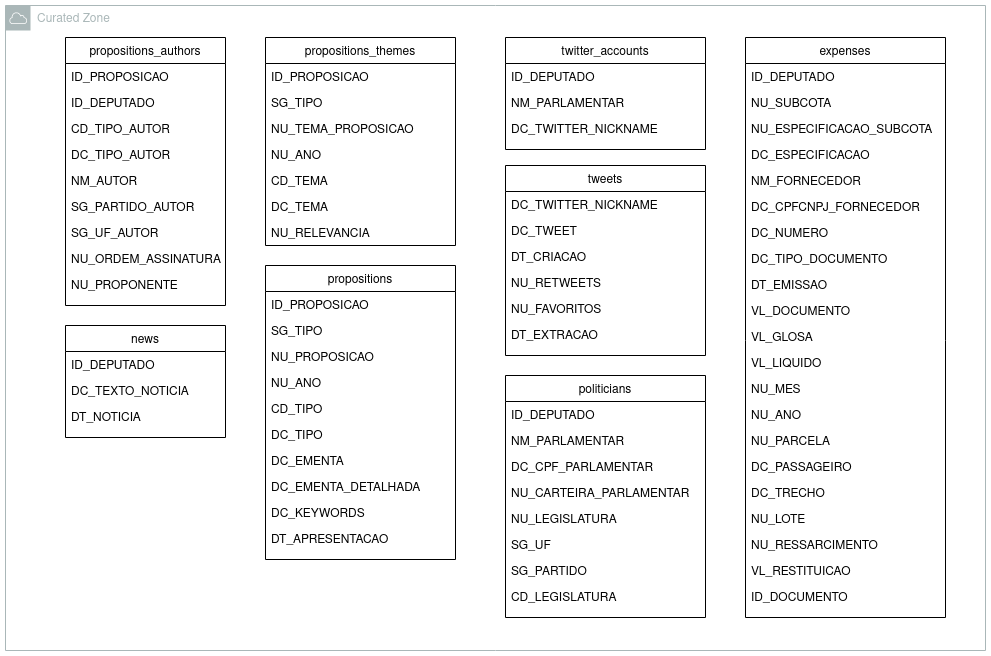
\includegraphics[width=.8\textwidth]{TCC/figuras/curated_zone.png}
	% Caption centralizada
% 	\captionsetup{justification=centering}
	% Caption e fonte
	 \vspace{-0.3cm}
	\\\textbf{\footnotesize Fonte: Elaborada pelo autor}
	\label{fig:tela1}
\end{figure}

Observa-se na figura 5 que todos os campos dos \textit{schemas} possuem um prefixo. Esse prefixo descreve a natureza do campo. Eles são definidos como: 

\begin{itemize}
\item \textbf{ID}: Identificador (inteiro);
\item \textbf{CD}: Código (\textit{string});
\item \textbf{DC}: Descrição (string);
\item \textbf{NM}: Nome (string);
\item \textbf{SG}: Sigla (string);
\item \textbf{NU}: Número (inteiro);
\item \textbf{VL}: Valor (decimal);
\item \textbf{DT}: Data (\textit{timestamp}).
\end{itemize}

\section{Análise exploratória de dados} Conforme descrito nas seções anteriores, todos os passos para extração e limpeza dos dados já foram realizados e, utilizando a \textit{Curated Zone}, os dados estão prontos para análise. Neste ponto, foram criados indicadores que descrevem as atividades parlamentares exercidas na Câmara dos Deputados, se tratando especificamente dos gastos dos parlamentares, os partidos políticos, proposições submetidas à Câmara com seus respectivos temas e status, além de categorizar as atividades dos políticos no Twitter e também as notícias que os citam no portal G1. Logo, tem-se um panorama geral onde pode-se identificar as reais atividades do deputado e compará-las com o seu discurso na mídia. Esse exercício comparativo foi realizado com uma amostra dos parlamentares existentes. Para essa análise, foram criadas 9 categorias, sendo elas: Cultura, Ciência, Trabalho, Saúde, Educação, Economia, Segurança Pública, Direitos Humanos e Desenvolvimento Urbano. Foram identificadas as proposições que possuem temas relacionados a essas categorias e também as atividades midiáticas dos parlamentares que se enquadram nesses grupos. Assim, um agrupamento foi realizado com granularidade a nível dos deputados contabilizando a quantidade de proposições e pronunciamentos para cada categoria, possibilitando a análise de correlação entre essas variáveis.